%%%%%%%%%%%%%%%%%%%%%%%%%%%%%%%%%%%%%%%%%%%%%%%%%%%%%%%%%%%%%%%%%%%%%%%%%%%%%%%%
%2345678901234567890123456789012345678901234567890123456789012345678901234567890
%        1         2         3         4         5         6         7         8

\documentclass[letterpaper, 10 pt, conference]{ieeeconf}  % Comment this line out
                                                          % if you need a4paper
%\documentclass[a4paper, 10pt, conference]{ieeeconf}      % Use this line for a4
                                                          % paper

\IEEEoverridecommandlockouts                              % This command is only
                                                          % needed if you want to
                                                          % use the \thanks command
\overrideIEEEmargins
% See the \addtolength command later in the file to balance the column lengths
% on the last page of the document

% The following packages can be found on http:\\www.ctan.org
%\usepackage{graphics} % for pdf, bitmapped graphics files
%\usepackage{epsfig} % for postscript graphics files
%\usepackage{mathptmx} % assumes new font selection scheme installed
%\usepackage{times} % assumes new font selection scheme installed
%\usepackage{amsmath} % assumes amsmath package installed
%\usepackage{amssymb}  % assumes amsmath package installed

\usepackage{graphics} % for pdf, bitmapped graphics files
\usepackage{graphicx}
\usepackage{epsfig} % for postscript graphics files
\usepackage{amsmath} % assumes amsmath package installed
\usepackage{amssymb}  % assumes amsmath package installed
\usepackage{amsfonts}
\usepackage{amsmath} % assumes amsmath package installed
\usepackage{subcaption}
\usepackage{cite}
\usepackage{color}
\usepackage{multirow}
\usepackage{algpseudocode,algorithm,algorithmicx}
%\usepackage{algorithm}
%\usepackage{algorithmicx}
%%\usepackage[]{algorithm2e}
%\usepackage{algcompatible}

%\SetKwInput{KwFind}{Find}


\title{\LARGE \bf
Robust Trajectory Planning for a Multirotor Using Funnel Library
}

%\author{ \parbox{3 in}{\centering Huibert Kwakernaak*
%         \thanks{*Use the $\backslash$thanks command to put information here}\\
%         Faculty of Electrical Engineering, Mathematics and Computer Science\\
%         University of Twente\\
%         7500 AE Enschede, The Netherlands\\
%         {\tt\small h.kwakernaak@autsubmit.com}}
%         \hspace*{ 0.5 in}
%         \parbox{3 in}{ \centering Pradeep Misra**
%         \thanks{**The footnote marks may be inserted manually}\\
%        Department of Electrical Engineering \\
%         Wright State University\\
%         Dayton, OH 45435, USA\\
%         {\tt\small pmisra@cs.wright.edu}}
%}

\author{Suseong Kim$^{1}$, Davide Falanga$^{1}$ and Davide Scaramuzza$^{1}$% <-this % stops a space
\thanks{*This work was not supported by any organization}% <-this % stops a space
\thanks{$^{1}$S. Kim is with the Robotics and Perception Group, University of Zurich, Switzerland
        {\tt\small $\{$suseong,falanga,sdavide$\}$ at ifi.uzh.ch}}%
}

\begin{document}

\maketitle
\thispagestyle{empty}
\pagestyle{empty}


%%%%%%%%%%%%%%%%%%%%%%%%%%%%%%%%%%%%%%%%%%%%%%%%%%%%%%%%%%%%%%%%%%%%%%%%%%%%%%%%
\begin{abstract}

This paper is about funnel library that can be used to generate robust trajectories for multirotors.

\end{abstract}


%%%%%%%%%%%%%%%%%%%%%%%%%%%%%%%%%%%%%%%%%%%%%%%%%%%%%%%%%%%%%%%%%%%%%%%%%%%%%%%%
\section{INTRODUCTION}

Throughout the paper, $0_{ij}$ stands for the zero matrix in $\mathbb{R}^{i\times j}$, and $I_i$ denotes the identity matrix in $\mathbb{R}^{i\times i}$. 
For a matrix, $\|\cdot\|$ represents the induced 2 norm, and $\lambda_{\max}(\cdot)$ and $\lambda_{\min}(\cdot)$ indicate the maximum and minimum eigenvalues.
Also, $|\cdot|$ is the Euclidean norm for a vector. 
For two vectors $\alpha,\beta \in \mathbb{R}^{3\times 1}$, 
we denote the inner and cross products as $\langle \alpha,\beta\rangle = \alpha^\top \beta$ and $\textbf{S}(\alpha)\beta = \alpha \times \beta$. 
For two quaternions $\mathbf{q}_1$ and $\mathbf{q}_2$, the quaternion multiplication expressed as $\mathbf{q}_1\otimes\mathbf{q}_2$. 
Also, $\textbf{P}(\cdot)$ is the quaternion representation of a vector $\omega\in\text{so}(3)$ such as $\textbf{P} = [0\;\omega^\top]^\top$. 
The rotation of a vector is indicated as $\mathbf{q}_1\odot\omega = \textbf{q}_1\otimes\textbf{P}(\omega)\otimes\textbf{q}_1^{-1}$. 
Furthremore, $\text{c}$ and $\text{s}$ are shorthands of $\cos$ and $\sin$, respectively.

\section{Quadrotor dynamics and control}

\subsection{Quadrotor dynamics}
To describe the dynamic model of a multirotor, we define the inertial $O_I\{x_I,y_I,z_I\}$ and the multirotor body-fixed $O_b\{x_b,y_b,z_b\}$ frames. The body-fixed frame is located at the center of the multirotor. 
The translational and angular dynamics of a multirotor is described as follows:
\begin{align}
\ddot{p} &= -gz_I + Tz_b + F_d + \delta \label{eq:translational} \\
\dot{\textbf{q}} &= \textstyle{\frac{1}{2}}\textbf{q}\otimes \text{P}(\omega) \label{eq:rotational}
\end{align}
where $p$ is the position of $O_b$ with respect to $O_I$, and $\textbf{q} = [q_0\;\bar{q}^\top]^\top$ is the unit quaternion describing the orientation of $O_b$ with respect to $O_I$.
The angular velocity of $O_b$ represented in $O_b$ is denoted as $\omega$.
The terms $g$ and $T$ are gravitational constant and mass normalized collective thrust, respectively. 
Without loss of generality, the axis $z_I$ is defined as $e_3 = [0\;0\;1]^\top$.
The rotor drag applied on the multirotor is denoted as $F_d$, and it is expressed as follows [IFAC]:
\begin{equation}
F_d = c_d\textbf{q}\odot\pi_z\textbf{q}^{-1}\odot \dot{p} \label{eq:rotorDrag}
\end{equation}
where $c_d$ is the rotor drag coefficient, and $\pi_z = I_3 - e_3^\top e_3$ is the matrix projecting a vector onto the $x_by_b$ plane.
The external forces and model uncertainties excluding the rotor drag term are lumped in $\delta \in \mathbb{R}^{3\times 1}$. 

In eq. \eqref{eq:rotational}, the angular velocity $\omega$ is used as the input term. 
It is possible based on the assumption that the multirotor body angular rate $\omega$ could be directly controlled as also supposed in [DANDREA].
Therefore, the input terms of the multirotor dynamics in eqs. \eqref{eq:translational} and \eqref{eq:rotational} are $T$ and $\omega$.
\\
\textbf{Uncertainty and disturbances}
In the free flight scenario which is not incorporating physical interaction with environment such as pushing or pulling, rotor and fuselage drag could be considered as the biggest external disturbances [DRAG].
XXXXX
Conclusion is that the rotor drag is not ignorable and proportional to the body velocity.
Other disturbances are small and can be assumed to be bounded to certain values.

\subsection{Multirotor control} \label{sec:controller}
Let us assume that the reference trajectory of the differential flat output[MEL] $\{p(t)^r,\psi^r(t)\}$ is given.
Here, $p^r(t)$ is the reference trajectory of the multirotor, and $\psi^r(t)$ represents the reference rotation of the multirotor about the $z_b$ body axis, i.e. yaw angle in the Euler angle representation.

To control the translational motion of a multirotor, we utilized a geometric control method [TYL] which is widely utilized in the researches on multirotors [RPG][UPENN][MIT].
Let $e_p = p - p^r$ and $e_v = \dot{p} - \dot{p}^r$ be the position and velocity error terms.
With the above definitions, the mass normalized thrust $T$ and desired thrust direction of a multirotor $z_b^d$ could be computed as the following procedure:
\begin{align}
\ddot{p}^{d} &= -K_p e_p - K_v e_v + ge_3 + \ddot{p}^r \label{eq:ddpd} \\
z_b^{d} &= \ddot{p}^{d}/|\ddot{p}^{d}| \nonumber \\
T &= \langle \ddot{p}^{d}, z_b \rangle = |\ddot{p}^{d}|\langle z_b^d, z_b \rangle \nonumber 
\end{align}
where $K_p$ and $K_v$ are gain matrices with positive diagonal entries.
By substituting the terms $T$ and $\ddot{p}^d$ in \eqref{eq:translational}, the error dynamics of the translational motion could be derived as follows:
\begin{align}
\ddot{e}_p &= -ge_3 + Tz_b + F_d + \delta - \ddot{p}^r + \ddot{p}^d - \ddot{p}^d \nonumber \\
&= -K_pe_p -K_ve_v + F_d + \delta + Tz_b - \ddot{p}^d \nonumber \\
&= -K_pe_p -K_ve_v + F_d + \delta + |\ddot{p}^d|\{\langle z_b^d, z_b \rangle z_b - z_b^d\} \nonumber \\
&= -K_pe_p -K_ve_v + F_d + \delta +  |\ddot{p}^d|\text{s}_\Phi u \label{eq:translationalError1}
\end{align}
where $\Phi$ is the angle between the axes $z_b$ and $z_b^d$, and $u$ is the unit vector indicating the direction of the term inside of the curly bracket.

Similarly, the rotational motion of a multirotor could be analyzed by combining it with a control law that generates the desired angular rate $\omega^d$. 
First, we compute the desired attitude of the multirotor with $\psi^r(t)$ and $z_b^d$ as follows: [MEL]
\begin{align}
\bar{y}_b &= [\begin{array}{ccc}-\text{s}_{\psi^r}&\text{c}_{\psi^r}&0\end{array}]^\top \nonumber \\
x_b^d &= \text{S}(\bar{y}_b)z_b^d / |\text{S}(\bar{y}_b)z_b^d | \nonumber \\ 
y_b^d &= \text{S}({z}_b^d)x_b^d / |\text{S}(z_b^d)x_b^d |. \nonumber  
\end{align}
Then, based on the axes $\{x_b^d,y_b^d,z_b^d\}$, the desired coordinate could be represented with the unit quaternion $\textbf{q}^d$. 
The attitude error between $\textbf{q}^d$ and $\textbf{q}$ is denoted as $\textbf{q}_e = \textbf{q}^{-1}\otimes \textbf{q}^d$. To decrease the attitude error $\textbf{q}_e = [q_e\;\bar{q}_e^\top]^\top$, the angular velocity is set as 
\begin{equation}
\omega = \left\{
\begin{array}{ll}
\omega_d^d - k_p \bar{q}_e & \text{if  }\;q_e \geq 0, \\ 
\omega_d^d + k_p \bar{q}_e & \text{if  }\;q_e < 0. \\ 
\end{array}
\right.
\end{equation}
where $\omega_d^d$ is the desired angular velocity of $\textbf{q}^d$ represented in $\textbf{q}^d$.
According to [ETH], the attitude error $\textbf{q}_e$ is globally asymptotically stable equilibrium point. 
Hence, it is possible to assume that the error $\Phi$ is also asymptotically stable, and bounded by a known value. NEEDS MORE EXPLANATIONS.
\\
\textbf{Assumption : }
In this work, we assume that the norm of the external disturbance is bounded as $|\delta| \leq \bar{\delta}$. 
Also, the norm of the nominal collective thrust is bounded as $|ge_3 + \ddot{p}^r| \leq \bar{T}$ given any $\mathcal{C}^2$ reference trajectory $x^r$.  
Furthermore, the norm of the thrust axis error is also bounded such as $|\text{s}_\Phi| \leq \bar{\text{s}}_\Phi$ with the attitude controller.

\subsection{Stability analysis} \label{sec:stabilityAnalysis}
In Sec. \ref{sec:controller}, it is assumed that the attitude error is bounded for all flight duration.
In this subsection, we investigate the stability of the translational dynamics in eq. \eqref{eq:translationalError1}.  

As the first step, the dynamics system is summarized as follows: 
\begin{equation}
\begin{array}{l}
\dot{e}_p = e_v \\
\dot{e}_v = -K_pe_p-K_ve_v+F_d+\delta+\text{s}_\Phi|\ddot{p}^d| u. 
\end{array} \label{eq:errorDynamics}
\end{equation}
To analyze the stability of the error dynamics conveniently, we assume that $K_p = k_pI_3$ and $K_v = k_vI_3$ with positive scalar gain values $k_p$ and $k_v$. 
Then, we define the Lyapunov candidate function as $\bar{V}=\frac{1}{2}e^\top \bar{P} e$ where $e = [e_p^\top\;e_v^\top]^\top$ and
\begin{equation}
\bar{P} = \left[
\begin{array}{rr}
(k_p+k_d)I_3 & I_3 \\ I_3 & I_3
\end{array}
\right]. \nonumber
\end{equation}
The Lyapunov function is positive definite when $k_p + k_v > 1$.
Furthermore, the directional derivative of $\bar{V}$ can be summarized as follows:
\begin{align}
\dot{\bar{V}} &= -k_p e_p^\top e_p -k_v e_v^\top e_v + e_v^\top e_v \nonumber \\
&\;\;\;\;+(e_p+e_v)^\top\{\delta + F_d + |\ddot{p}^d|\text{s}_\Phi u\}.
\end{align}
Then, by having $\ddot{p}^d$ in eq. \eqref{eq:ddpd}, $|\delta|\leq\bar{\delta}$, $|F_d| \leq c_d|\dot{p}^r+e_v|$, and $|\text{s}_\Phi u| < \bar{\text{s}}_\Phi$, the above relation is rearranged further as
\begin{align}
\dot{\bar{V}} &\leq -k_p|e_p|^2 -(k_v+1)|e_v|^2 +(|e_p| + |e_v|)\nonumber \\
&\;\;\;\;\times\{\bar{\delta} + c_d|\dot{p}^r+e_v|+\bar{\text{s}}_\Phi(|-k_pe_p-k_ve_v|+\bar{T})\} \nonumber \\
&\leq -\bar{e}^\top \bar{Q}\bar{e} + \Delta|\bar{e}| \label{eq:dotV}
\end{align} 
where $\bar{e} = [|e_p|\;|e_v|]^\top$, $\Delta = \bar{\delta}+c_d|\dot{p}^r|+\bar{s}_\Phi\bar{T}$ and
\begin{align}
\bar{Q} &= \left[
\begin{array}{rr}
k_p(1-\bar{s}_\Phi) & -\frac{1}{2}\{c_d+\bar{s}_\Phi(k_p+k_d)\} \\
-\frac{1}{2}\{c_d+\bar{s}_\Phi(k_p+k_d)\} & k_v(1-\bar{s}_\Phi)-1-c_d
\end{array}
\right].\nonumber 
\end{align}
Here, the matrix $\bar{Q}$ can be considered as the summation of the two separated parts such as $\bar{Q} = Q_A + \bar{\text{s}}_\Phi Q_B$ where
\begin{align}
Q_A &= \left[
\begin{array}{rr}
k_p & -\frac{1}{2}c_d \\ -\frac{1}{2}c_d & k_v-1-c_d
\end{array}
\right] \nonumber \\
Q_B &= \left[
\begin{array}{rr}
-k_p & -\frac{1}{2}(k_p+k_v) \\ -\frac{1}{2}(k_p+k_v) & -k_v
\end{array}
\right].
\end{align}
By setting $k_v > 1+c_d$ and $k_p > \frac{c_d^2}{4(k_v-1-c_d)}$, we can make the matrix $Q_A$ positive definite. 
On the other hand, the matrix $Q_B$ cannot be positive definite since $\text{det}(Q_B) = -\frac{1}{4}(k_p-k_v)^2 \leq 0$, i.e. $\lambda_{\max}(Q_B)\geq0$ and $\lambda_{\min}(Q_B)\leq 0$.
However, even though $Q_B$ is not positive definite, we can assure that the matrix $\bar{Q}$ is positive definite with the condition $\bar{\text{s}}_\Phi < -\lambda_{\min}(Q_A)/\lambda_{\min}(Q_B)$
which could readly be achieved since $\bar{\text{s}}_\Phi \approx 0$ with a well designed attitude controller.
Therefore, with the gain values $k_p$ and $k_v$ fulfilling $\lambda(\bar{Q}) \geq 0$, eq. \eqref{eq:dotV} becomes
\begin{align}
\dot{V} &\leq -\lambda_{\min}(\bar{Q})|\bar{e}|^2 + \Delta|\bar{e}| \nonumber \\
&\leq -\lambda_{\min}(\bar{Q})(1-\theta)|\bar{e}|^2-\lambda_{\min}(\bar{Q})\theta|\bar{e}|^2 + \Delta|\bar{e}| \nonumber
\end{align}
where $0<\theta<1$.
Finally,
\begin{equation}
\dot{\bar{V}} \leq -\lambda_{\min}(\bar{Q})(1-\theta)|\bar{e}|^2, \text{ where } |\bar{e}| \geq \frac{\Delta}{\lambda_{\min}(\bar{Q})\theta}. \nonumber
\end{equation}
Therefore, the error dynamics of the translational system of a multirotor is uniformly ultimately bounded. Furthermore, the ultimate bound $b$ could be computed as 
\begin{equation}
b = \sqrt{\frac{\lambda_{\max}(\bar{P})}{\lambda_{\min}(\bar{P})}\mu^2},\;\;\;
\mu = \frac{\Delta}{\lambda_{\min}(\bar{Q})\theta}. 
\label{eq:expected}
\end{equation}

In this analysis, we can see that any error will eventually enter into the ultimate bound with radius $b$ within finite time. 
The ultimate bound is the function of $\Delta$ and it is the combination of $\bar{\delta}$, $|\dot{p}^r|$, and $\bar{T}$. Also, the drag coefficient $c_d$ and the maximum attitude error $\bar{\text{s}}_\Phi$ could be interpreted as the weight terms. 
Hence, the radius of the bound will get bigger by having larger values of disturbances, reference velocity, and reference acceleration ($\bar{T} = |ge_3 + \ddot{p}^r|$). 

However, even though we could get the general sense on how the error will behave, 
it is difficult to know the tight ultimate bound that the error states actually resides. 
Also, given initial set of error states, it is hard to see how the error will evolve before getting into the ultimate bound.

\section{Computing funnels}
In Sec. \ref{sec:stabilityAnalysis}, we checked the general behavior of the translational error dynamic system via classical Lyapunov stability analysis.
Furthermore, with sum of squares optimization tools, we can compute the reachable set of the state $e$.
The concept of funnel and numerical method for computing funnel can be referred to [MAJ1,MAJ2]. 

\subsection{Concept of funnel}
Funnel $\mathcal{F}(t) \subset \mathbb{R}^{6\times 1}$  represents the reachable set of error $e(t)\in \mathbb{R}^{6\times 1}$ given the initial set of error $e(0) \in \xi_0$ and a closed-loop dynamic equation.
In other words, the error $e(0)$ contained in the set $\xi_0$ will evolve only inside of the set $\mathcal{F}(t)$ for $t\geq 0$.
These property of the funnel could be written as follows:
\begin{equation}
e(0) \in \xi_0,\;\xi_0 \subset \mathcal{F}(0)\;\Rightarrow\; e(t) \in \mathcal{F}(t),\;\;\forall t \geq 0. \label{eq:funnel1}
\end{equation}

Define a time varying positive definite matrix $P(t) \in \mathbb{R}^{6\times 6}$, a positive scalar variable $\alpha(t)$, and $V(t,e) = e(t)^\top P(t) e(t)$.
In the following analysis, $V(t,e)$ will be the Lyapunov function, and $\alpha(t)$ will be the parameter indicating the level of $V(t,e)$.
Then, we represent the set $\mathcal{F}(t)$ as 
\begin{equation}
\mathcal{F}(t) = \{e(t) \in \mathbb{R}^{6\times 1} | V(t,e) \leq \alpha(t)\} \label{eq:funnel2}
\end{equation}
where $V$ and $\alpha$ are constrained such that
\begin{align}
&\dot{V}(t,\hat{e}) < \dot{\alpha}(t) \label{eq:funnel3} \\
&\text{for }\;\;\;\hat{e}(t) = \{e(t)|V(t,e) = \alpha(t),\;t\in[0,\infty)\}. \nonumber
\end{align}
From the constraint, it is obvious that the state $e(t) \in \mathcal{F}(t)$ cannot escape the sublevel set described by $V(t,e) \leq \alpha(t)$.
Therefore, the set $\mathcal{F}(t)$ defined in eqs. \eqref{eq:funnel2} and \eqref{eq:funnel3}
 complies with the definition of funnel in eq. \eqref{eq:funnel1} [MAJ]. 

Another constraint to fulfill the property of funnel defined in eq. \eqref{eq:funnel1} is related to the initial condition of a funnel. 
The initial set of $e(0)$, i.e. $\xi_0$, should be the subset of $\mathcal{F}(0)$. 
To enforce the constraint, we define $\xi_0 = \{e|e^\top R e \leq 1\}$ with a positive definite matrix $R$. Then, the constraint can be written as follows:
\begin{equation}
V(0,\hat{e}) \leq \alpha(0)\;\text{ for }\;\hat{e} = \{e |e^\top R e \leq 1\}.
\end{equation} 

Furthermore, we want to find $V$ and $\alpha$ that represent the reachable set of $e$ small to make the funnel as less consertative as possible. 
Since $P$ is a positive definite matrix and $V$ is a quadratic function of $e$, 
it is possible to define an ellipsoid that enclosing the set of error $e=\{e|V(e,t) = \alpha(t) \}$.
Then, by minimizing the volume of the enclosing ellipsoid, the size of the funnel could be minimized consequently.
The outer ellipsoid can be formulated such as
\begin{align}
&\hat{e}^\top(t) S(t) \hat{e}(t) \leq 1  \nonumber \\
&\text{ for }\;\;\;\hat{e}(t) = \{e(t)|V_\mathcal{F}(t,e) = \alpha(t),\;t \in [t_0,t_f]\}. \nonumber
\end{align}
where $S(t)\in \mathbb{R}^{6\times 6}$ is the positive definite matrix representing the shape of the outer shell ellipsoid. Note that the volume of the ellipsoid is proportional to the determinant of $S(t)$.

Based on these observations, we can formulate the optimization problem to find the funnel as follows:
\begin{equation}
\begin{array}{rl}
\displaystyle{\inf_{P,\alpha,S}} & \int_{t_0}^{t_f} \det{S(t)}\text{d}t \label{eq:optim1} \\
\displaystyle{\text{s.t.}}& \dot{V}(t,\hat{e}) < \dot{\alpha}(t)\text{ for }\hat{e} = \{e(t)|V(t,e) = \alpha(t)\}, \nonumber \\
& \hat{e}^\top S(t) \hat{e} \leq 1\text{ for }\hat{e} = \{e(t)|V(t,e) = \alpha(t)\}, \nonumber \\
& V(t_0,\hat{e}) \leq \alpha(t_0)\text{ for }\hat{e} = \{e|e^\top R e \leq 1\}. \nonumber
\end{array}
\end{equation}

\subsection{Computing funnel} \label{sec:computeFunnels}
We compute the funnel for the multirotor translational error dynamic system.
First of all, 
we define the Lyapunov function in the quadratic form such as $V = e(t)^\top P(t) e(t)$ with the time varying positive definite matrix
\begin{equation}
P(t) = \left[
\begin{array}{cc}
P_p(t) & P_{pv}(t) \\
P_{pv}(t) & P_v(t)
\end{array}
\right] \label{eq:funnelP}
\end{equation}
where $P_p(t)$, $P_{pv}(t)$, and $P_v(t)$ are diagonal matrices with positive entries.
Then, with eq. \eqref{eq:errorDynamics}, the directional derivative of the Lyapunov function $V$ is rearranged as follows: 
\begin{align}
\dot{V} &= -e^\top ( A^\top P + PA) e + e^\top \dot{P}e \nonumber \\
&\;\;\;\;+2e^\top P B(\delta+\text{s}_\Phi|\ddot{p}^d|{u}+F_d) \nonumber
\end{align}
where
\begin{equation}
A = \left[
\begin{array}{rr}
0_{33} & I_3 \\ -K_p & -K_d 
\end{array}
\right],\;\;\;B = \left[
\begin{array}{r}
0_{33} \\ I_3
\end{array}
\right].\nonumber 
\end{equation}
In the right hand side of the above equation, the third term further developed as
\begin{align}
&e^\top P B(\delta+\text{s}_\Phi|-K_p e_p -K_v e_v + ge_3 + \ddot{p}^r|\bar{u}+F_d) \nonumber \\
&\leq |e^\top P B|\{\bar{\delta} + \bar{\text{s}}_\Phi(k_p|e_p| + k_v|e_v| + \bar{T})+c_d|\dot{p}^r+e_v|\} \nonumber \\
&\leq (p_{pv}|e_p|+p_v|e_v|)\{\bar{\text{s}}_\Phi(k_p|e_p|+k_v|e_v|)+c_d|e_v|+\Delta\}\label{eq:deltaConst}
\end{align}
where $p_{pv}$, $p_v$, $k_p$, and $k_v$ are maximum eigenvalues of $P_{pv}$, $P_v$, $K_p$, and $K_v$.
Also, $\Delta = \bar{\delta}+c_d|\dot{p}^r| + \bar{\text{s}}_\Phi\bar{T}$.
To handle the error states with the norm, i.e. $|e_p|$ and $|e_v|$, we define two variables $\bar{e}_p\in\mathbb{R}$ and $\bar{e}_v\in\mathbb{R}$ satisfying the following constraints:
\begin{equation}
\begin{array}{ll}
\bar{e}_p^2 = e_p^\top e_p = |e_p|^2, & \bar{e}_p \geq 0 \\
\bar{e}_v^2 = e_v^\top e_v = |e_v|^2, & \bar{e}_v \geq 0. \\
\end{array} \nonumber 
\end{equation} 
Then, $\dot{V}$ is further developed as follows:
\begin{align}
\dot{V} &\leq -e^\top( PA + A^\top P) e + e^\top \dot{P}e  \label{eq:aaa}\\
 &\;\;\;\;+2(p_{pv}\bar{e}_p+p_v\bar{e}_v)\{\bar{\text{s}}_\Phi(k_p\bar{e}_p+k_v\bar{e}_v) + c_d\bar{e}_v + \Delta\}. \nonumber 
\end{align}

In $V$ and $\dot{V}$, the variables of the optimization problem are continuous in $t$. 
To solve the problem in more efficient manner, 
we discretized variables $P$, $\alpha$, and $S$ in $t$.
The discretized time is denoted as $t_n\;(n=0,\cdots,N)$. 
Then, the optimization problem can be reformulated as the following:
\begin{figure*}[t]
\begin{subfigure}[b]{0.5\textwidth}
\centering
\includegraphics[width=8.5cm]{s2b_ver3.pdf}
\caption{Funnels computed with the initial region with $\xi^s$.}
\end{subfigure}
\begin{subfigure}[b]{0.5\textwidth}
\centering
\includegraphics[width=8.5cm]{b2s_ver3.pdf}
\caption{Funnels computed with the initial region with $\xi^b$.}
\end{subfigure}
\caption{
Funnels computed with various values of $\Delta_k$ and $\xi_0$. The detailed parameters and settings are available in table. \ref{table:settings}. The black solid and dotted lines are with $\Delta_l = 0.5$ and $1.0$, the blue solid and dotted lines are with $\Delta_l = 1.5$ and $2.0$, and the green solid and dotted lines are $\Delta_l = 2.5$ and $3.0$.}
\label{fig:funnelSamples}
\end{figure*}

\begin{align}
&
\begin{array}{rl}
\displaystyle{\inf_{P(t_n),\alpha(t_n),S(t_n),p_{pv}(t_n),p_v(t_n)}} & \displaystyle{\sum_{n=0}^{N}} \det(S(t_n))  \\
\end{array} \label{eq:optim2} \\
&
\begin{array}{rl}
\displaystyle{\text{s.t.}}& \dot{\alpha}(t_n) - \dot{V}(t_n) \geq 0\text{ with constraints $c_1$ to $c_9$},  \\
& 1-e^\top S(t_n) e \geq 0\text{ with constraints $c_9$ and $c_{10}$}, \nonumber \\
& \alpha(t_0) - V(t_0) \geq 0\text{ with constraint $c_{11}$}. \nonumber
\end{array} \nonumber 
\end{align}
where
\begin{equation}
\begin{array}{rlrl}
c_1:& \bar{e}_p^2 = e_p^Te_p,           & c_2:&\bar{e}_p \geq 0 \\
c_3:& \bar{e}_v^2 = e_v^Te_v,           & c_4:&\bar{e}_v \geq 0 \\
c_5:& p_{pv}(t_n)I_3 \geq P_{pv}(t_n),      & c_6:&p_{pv}(t_n)I_3 \geq -P_{pv}(t_n) \\
c_7:& p_{ v}(t_n)I_3 \geq P_{ v}(t_n),      & c_8:&p_{ v}(t_n)I_3 \geq -P_{ v}(t_n) \\
c_9:& \alpha(t_n) - V(t_n) = 0, & c_{10}:&S(t_n) > 0 \\
c_{11}:& 1-e^\top R e = 0. &&
\end{array} \nonumber
\end{equation}
The constraints $c_5$ to $c_8$ is added to ensure
 $p_{pv}(t_n) \geq \|P_{pv}(t_n)\|$ and $p_v(t_n) \geq \|P_v(t_n)\|$ 
with diagonal matrices $P_{pv}(t_n)$ and $P_v(t_n)$.
In addition, $\dot{P}(t_n)$ and $\dot{\alpha}(t_n)$ could be implemented as
\begin{equation}
\begin{array}{cc}
\dot{P}(t_n) = \frac{P(t_{n+1}) - P(t_n)}{\text{d}t}, & \dot{\alpha}(t_n) = \frac{\alpha(t_{n+1})-\alpha(t_n)}{\text{d}t}. 
\end{array} \label{eq:dt}
\end{equation}
The optimization problem in eq. \eqref{eq:optim2} could be transformed into the form of sum of squares problem and solved efficiently by referring [MAJ].

\subsection{Funnel library}
In the optimization problem, the list of parameters are~: the initial set of error states $\xi_0$; 
the gain matrices $K_p$ and $K_d$; 
the norm of maximum attitude angle error $\bar{\text{s}}_\Phi$;
the rotor drag coefficient $c_d$; and the lumped disturbance term $\delta$. 
Among these parameters, the gain matrices are manually set by an operator to satisfy the required flight performance in accordance with applications. 
The attitude error $\bar{\text{s}}_\Phi$ and drag coefficient $c_d$ terms should be seleceted to be comparable with respect to the actual values of the multirotor.
Accordingly, the terms $K_p$, $K_d$, $c_d$, and $\bar{\text{s}}_\Phi$ can be set with the current setting of the multirotor.
However, the lumped disturbance term $\Delta(=\bar{\delta}+c_d|\dot{p}^r|+\bar{\text{s}}_\Phi|ge_3 + \ddot{p}^r|)$ keeps changing while a multirotor is in flight. 
For example, the external disturbance, e.g. wind condition, could be different location to location.
Also, the reference velocity $\dot{p}^r$ and accelerations $\ddot{p}^r$ are derived from the reference trajectory so that the terms $|\dot{p}^r|$ and $|ge_3+\ddot{p}^r|$ will change while the multirotor is in maneuver.
According to the stability analysis in eq. \eqref{eq:expected}, 
the radius of the ultimate bound varies proportionally with $\Delta$, 
and the behavior of the error states will also be altered with respect to $\Delta$. 
Therefore, we generate \textit{library of funnels} with various values of $\Delta$, which will be denoted as $\Delta_l$ with $l(=1,\cdots,L)$ to use them depending on the magnitude of $|\Delta|$.
%For example, if the external force $\delta$ is available apriori, 
%the terms $|\dot{p}^r|$ and $|ge_3 + \ddot{p}^r|$ are directly computable with the reference trajectory. 
%Therefore, we can guess the $\Delta$ along the reference trajectory and look up the library of funnel to compute how the error state will behave.

Let $U_{\Delta_l}$ represent the set of ultimate bound when the norm of disturbance is $\Delta_l$.
For each $\Delta_l$, we evaluate the funnel with two different settings of initial sets such that $U_{\Delta_l}\subset\xi_b$ and $\xi_s\subset U_{\Delta_l}$.
By doing this, we can see how the error states behave until they reach their ultimate bound from both smaller and larger regions.

\begin{table}[b]
\begin{center}
\begin{tabular}{|r|l||r|l|} 
\hline
param & value & param & value \\ \hline \hline
$\text{d}t$ & 0.05 [s] & $N$ & 100 \\ \hline
$K_{p,x}$ & 10 [s$^\text{-2}$] & $K_{v,x}$ & 4 [s$^\text{-1}$] \\ \hline
$K_{p,y}$ & 10 [s$^\text{-2}$] & $K_{v,y}$ & 4 [s$^\text{-1}$] \\ \hline
$K_{p,z}$ & 15 [s$^\text{-2}$] & $K_{v,z}$ & 6 [s$^\text{-1}$] \\ \hline
\multirow{2}{*}{$\bar{\text{s}}_\Phi$} & 0.0532[$\cdot$] & \multirow{2}{*}{$R_b\;(\xi_b)$} & blockdiag($1.56I_3,0.11I_3$) \\ 
& $\approx\sin3^\circ$ & & \;\;\;\;\;\;\;\;\;\;\;\;\;\;\;\;\;\; [$m^\text{-2}$, $m^\text{-2}s^\text{2}$] \\ \hline
$c_d$ & 0.32 [$s^\text{-1}$]                         & $R_s\;(\xi_s)$ & blockdiag($100I_3,11.1I_3$) \\ \hline
\end{tabular}
\caption{parameters used for computing funnel library} \label{table:settings} 
\end{center}
\end{table}

In summary, a funnel library is organized as the set such as ${F}_{\text{lib}} = \{F_{\Delta_1},\cdots,F_{\Delta_{l_M}}\}$.
Each element is evaluated with different value of disturbance $\Delta_l$, 
and it is constructed with funnels two different set of initial conditions as $F_{\Delta_l} = \{F_{\Delta_l}^b,F_{\Delta_l}^s\}$ where the superscript $j \in \{b,s\}$ indicates the initial condition $\{\xi_b,\xi_s\}$. The elements are the sequence of compact sets such as $F_{\Delta_l}^j = \{F_{\Delta}^j(t_0),\cdots,F_{\Delta}^j(t_N)\}$ where
\begin{equation}
F_{\Delta_l}^j(t_n) = \{e| e^\top P_{\Delta_l}^j(t_n) e \leq  \alpha_{\Delta_l}^j(t_n)\}. \label{eq:discreteFunnel}
\end{equation}
Here, $P_{\Delta_l}^j(t_n)$ and $\alpha_{\Delta_l}^j(t_n)$ are the parameters of the Lyapunov function eq. \eqref{eq:aaa} optimized in the funnel generation.
Then, a piece of funnel in the library is quoted as $F_{\Delta_l}^j(i)$ where $i$ indicates the sequence number, i.e. $t_n$, of funnel generated with the setting $\Delta_l$ and $j$.

As an example, we have generated funnels with the setting in table \ref{table:settings}.
Funnels are displayed with the $\Delta_l$ for every $0.5$ from $0.5$ to $3.0\;[m s^\text{-2}]$. 
The computed funnels are displayed in Fig. \ref{fig:funnelSamples}.
The funnel, which is ellipsoid, is projected to each coordinate for visualization purposes.
There are two notable characteristics from the generated funnels shown in fig. \ref{fig:funnelSamples}. 
First, if the disturbance $\Delta_l$ is set to the same value, the funnels converges to the similar values regardless of the initial condition $j$.
The second one is that the ultimate bounds of the each axis are proportional to the value of $\Delta_l$. 
These are the expected result from the analysis in eq. \eqref{eq:expected}.

\subsection{Combining funnels}
\begin{figure}[t]
\centering
\includegraphics[width=8cm]{funnel_combine.pdf}
\caption{Concept figure to explain how to connect funnels.}
 \label{fig:combiningConcept}
\end{figure}

In sec. \ref{sec:computeFunnels}, we described the method how to generate funnels with various fixed disturbance norm values.
However, the disturbance $\Delta(t)$ will keep varying with respect to time in most of flight operation scenarios.
Let us assume that we use only one funnel computed with $\Delta_l$ satistying $|\Delta(t)| \leq \Delta_l$ for $t>0$.
In this case, the funnel analysis will indicate that set of error will eventually converge to the ultimate bound with $|\Delta| = \Delta_l$. 
Then, the selected funnel will be too conservative since the size of the ultimate bound is proportional to the norm of disturbance.
Hence, in this subsection, we present the method for applying the funnel library computed with the fixed values of $\Delta_l$ to the general cases with time varying $\Delta(t)$. 
\begin{algorithm}[t]
  \caption{Assigning funnels along reference trajectory
    \label{alg:funnel}}
  \begin{algorithmic}[1]
    \Statex
    \Function{Combine Funnels }{$\Delta(t)$, $\xi_o$, $\mathcal{F}$}
	\State \textbf{find }$\Delta_{l}$\textbf{ s.t.} $\Delta_{l-1} < \Delta(0) \leq \Delta_l$
	\State $\Delta_{0} \gets \Delta_l$
	\State \textbf{find $t_n$ and $j$ with smallest volume of} $\bar{F}$  \textbf{s.t.}
	\State $\bar{F}=\{F|\xi_0 \subset F,\;F\in F_{\Delta_0}\}$
	\State $i_0 \gets t_n$ (\text{index of }$\bar{F}$)
	\State $j_0 \gets j$ (\text{initial condition of }$\bar{F}$)
      \For{$m \gets 1 \textrm{ to } M$}
				\State \textbf{find }$\Delta_l$\textbf{ s.t. } $\Delta_{l-1} < \hat{\Delta} \leq \Delta_l$
				\State \text{where} $\hat{\Delta} = \max(\Delta(t)),\;\forall t\in[t_{m},t_{m+1}]$
				\State $\Delta_{m} \gets \Delta_l$
%				\If{$\Delta_m = \Delta_{m-1}$}
%				\State $i_m \gets i_{m-1}+1$, $j_m \gets j_{m-1}$
%				\Else
				\State \textbf{find $t_n$ and $j$ with smallest volume of} $\bar{F}$ \textbf{s.t.}  
				\State $\bar{F}=\{F|F_{\Delta_{m-1}}^{j_{m-1}}(i_{m-1}+1) \subset {F},\;F \in F_{\Delta_m}\}$
				\State $i_m \gets t_n$, $j_m \gets j$
%				\EndIf
      \EndFor
      \State \Return{$\Delta_m$, $j_m$, $i_m$ for $m=\{1,\cdots,M\}$}
    \EndFunction
  \end{algorithmic}
\end{algorithm}

In accordance with the funnel computation, we discretized the flight time with the same $\text{d}t$ used in eq. \eqref{eq:dt}.
Let denote the descritezed time as ${t}_m$ $(m = 0,\cdots,M)$.
Then, our approach for generating funnel with the time varying disturbance is assigning $i_m$, $j_m$, and $\Delta_m$ to quote $F_{\Delta_{m}}^{j_m}(i_m)$ for all discretized time $t_m$ during the flight. 

First of all, we explain the method for deciding the disturbance level $\Delta_l$ for $t \in [t_{m},t_{m+1}]$ which will be denoted as $\Delta_m$.
Among all $\Delta_l$ values, the obvious choice would be using the minimum one satisfying $|\Delta(t)| \leq \Delta_l$ during $t\in[t_{m},t_{m+1}]$. It is because that $\Delta_l$ is the closest to the actual $|\Delta(t)|$ as well as the condition required in eq. \eqref{eq:deltaConst} is satisfied.
If the step size between $\Delta_l$ and time intervals are discretized fine enough, the actual disturbance will be well reflected. 
This procedure is described in the first row of the fig. \ref{fig:combiningConcept}.

Secondly, with the selected disturbance level $\Delta_m$, we present the method for picking the indices $i_m$ and $j_m$. For further explanations, for now, we assume that $\Delta_{m-1}$, $i_{m-1}$, and $j_{m-1}$ are given.
Once we have $F_{\Delta_{m-1}}^{j_{m-1}}(i_{m-1})$, the set of error states at $t_m$ can be directly accessible from the funnel library by referring $F_{\Delta_{m-1}}^{j_{m-1}}(i_{m-1}+1)$. 
Then, we can find $\bar{F} \in F_{\Delta_m}$ satisfying $F_{\Delta_{m-1}}^{j_{m-1}}(i_{m-1}+1) \subset \bar{F}$.
It means that the set of error defined with $F_{\Delta_{m-1}}^{j_{m-1}}(i_{m-1})$ will evolve and be the subset of $\bar{F}$ at $t_m$. 
Accordingly, it is possible to assign any combination of $i_m$ and $j_m$ indicating elements of $\bar{F}$.
However, because we are interested in evaluating the reachable set as tight as possible, we choose $i_m$ and $j_m$ indicating $F_{\Delta_m}^{j_m}(i_m)$ with the smallest volume. 
Selecting the smallest volume funnel could be easily done since the volume of an ellipsoid is proportional to the determinant of the ellipsoid defined in eq. \eqref{eq:discreteFunnel}. 

So far, we explained the method how to find $F_{\Delta_m}^{j_m}(i_m)$ for $t_m$. In actual scenario, at $t_0$, $\Delta_0$ can be computed in the same manner and the initial set of error $\xi_0$ can act a role same as $F_{\Delta_{m-1}}^{j_{m-1}}(i_{m-1}+1)$.
Therefore, we can select funnels in the library from $t_0$ to $t_M$ in order.
The overall procedure is summarized in the algorithm 1.

\noindent\textbf{Note.} 
To implement the algorithm, we have to make the routine to check whether the condition $F_1 \subset F_2$ is true or false where the the sets $F_1 = \{e|e^\top R_1 e \leq 1\}$ and $F_2 = \{e|e^\top R_2 e \leq 1\}$ and  $R_1$ and $R_2$ are positive definite matrices.
In $F_1$ and $F_2$, the center of the ellipsoids are coincident at zero. 
Since the sets are defined as quadratic functions,
we can show that $F_1 \subset F_2$ is satisfied when $\lambda_{\max}(D_1^{-1}R_2D_1^{-\top} )\leq~1$ where $D_1$ is the Cholesky decomposition of $R_1( = D_1D_1^\top)$.

\subsection{Funnel for checking robustness of reference trajectories}
Once we generate the funnel library and combination of funnel pieces around the reference trajectory, the reachable set of multirotor position and velocity could be computed. Since we are particularly interested in checking the robustness of the reference trajectory, we focus on computing the reachable set of position.
As in eq. \eqref{eq:discreteFunnel}, a piece of funnel could be represented with the inequality 
\begin{equation}
F_{\Delta_m}^{j_m}(i_m) = \{e|e^\top P_{\Delta_m}^{j_m}(i_m)e \leq \alpha_{\Delta_m}^{j_m}(i_m)\}. \nonumber
\end{equation} 
Let $P_m = P_{\Delta_m}^{j_m}(i_m) / \alpha_{\Delta_m}^{j_m}$, and, from eq. \eqref{eq:funnelP}, the structure of $P_m$ is
\begin{equation}
P_m = \left[
\begin{array}{cc}
P_{m,p} & P_{m,pv} \\
P_{m,pv} & P_{m,v} 
\end{array}
\right]. \nonumber
\end{equation}
Then, the set of translational error, including position and velocity erros, can be projected into the position error ellipsoid such as
\begin{equation}
e_p^\top (P_{m,p} - P_{m,pv}^2 P_{m,v}^{-1}) e_p = 1. \label{eq:positionError}
\end{equation}
Therefore, for each $n$, the set of position can be evaluated with $e_p$ satisfying eq. \eqref{eq:positionError} such as $p_m = p^r(t_m) + e_p$.  

For example, let us define the position of a point on an obstacle as $p_\text{obs}$ and the parameter $\eta$ as 
\begin{equation}
\eta = (p_\text{obs}-p^r(t_m))^\top (P_{m,p} - P_{m,pv}^2 P_{m,v}^{-1})(p_\text{obs}-p^r(t_m)). \nonumber
\end{equation}
If $\eta \leq 1$, the point on the obstacle is inside of the reachable set of the position., Consequently, there will be a possibility of collision between the multirotor and the obstacle. On the other hands, if $\eta > 1$, the funnel analysis guarantees that the collision will not happen. 

%\section{Simulations}
%Monte Carlo simulation will be inserted to show that the funnel can encapsulate the error trajectories as supposed. 
%\subsection{Simulation setup}
%Simulation setup will be explained. Environment would be the Gazobo integrated with RotorS UAV simulator which explicitely incorporating the rotor drag terms.
%Multirotor will follow the minimum snap trajectories generated with to connect randomly generated waypoints.
%The initial condition is also randomly generated inside of the ultimate bound. 
%Hence, the goal of the simulation is to show that the trajectories starting inside of the ultimate bound (evaluated with the computed funnel) cannot escape the ultimate bound.
%\subsection{Simulation results}
%Plan is to giving explanation with the following style figure \ref{fig:simulation}
%\begin{figure}
%\centering
%\includegraphics[width=9cm]{monteCarlo.pdf}
%\caption{The green ellipse is the ultimate bound projected to each coordinate. 
%Since the gains $K_{p,x}$ and $K_{p,y}$, and $K_{v,x}$ and $K_{v,y}$ are set to same values, errors on $x$ and $y$ coordinates are displayed in the same figure.} \label{fig:simulation}
%\end{figure}

\section{Experiments}
Experimental scenario is the following. 
We want to find the \textit{safe} velocity that a multirotor can go through a pipe type object as shown in fig. \ref{fig:experimentalResult}.

\subsection{Experimental setup}
\subsection{Experimental results}
\begin{figure*}[!h]
\begin{subfigure}[b]{0.5\textwidth}
\centering
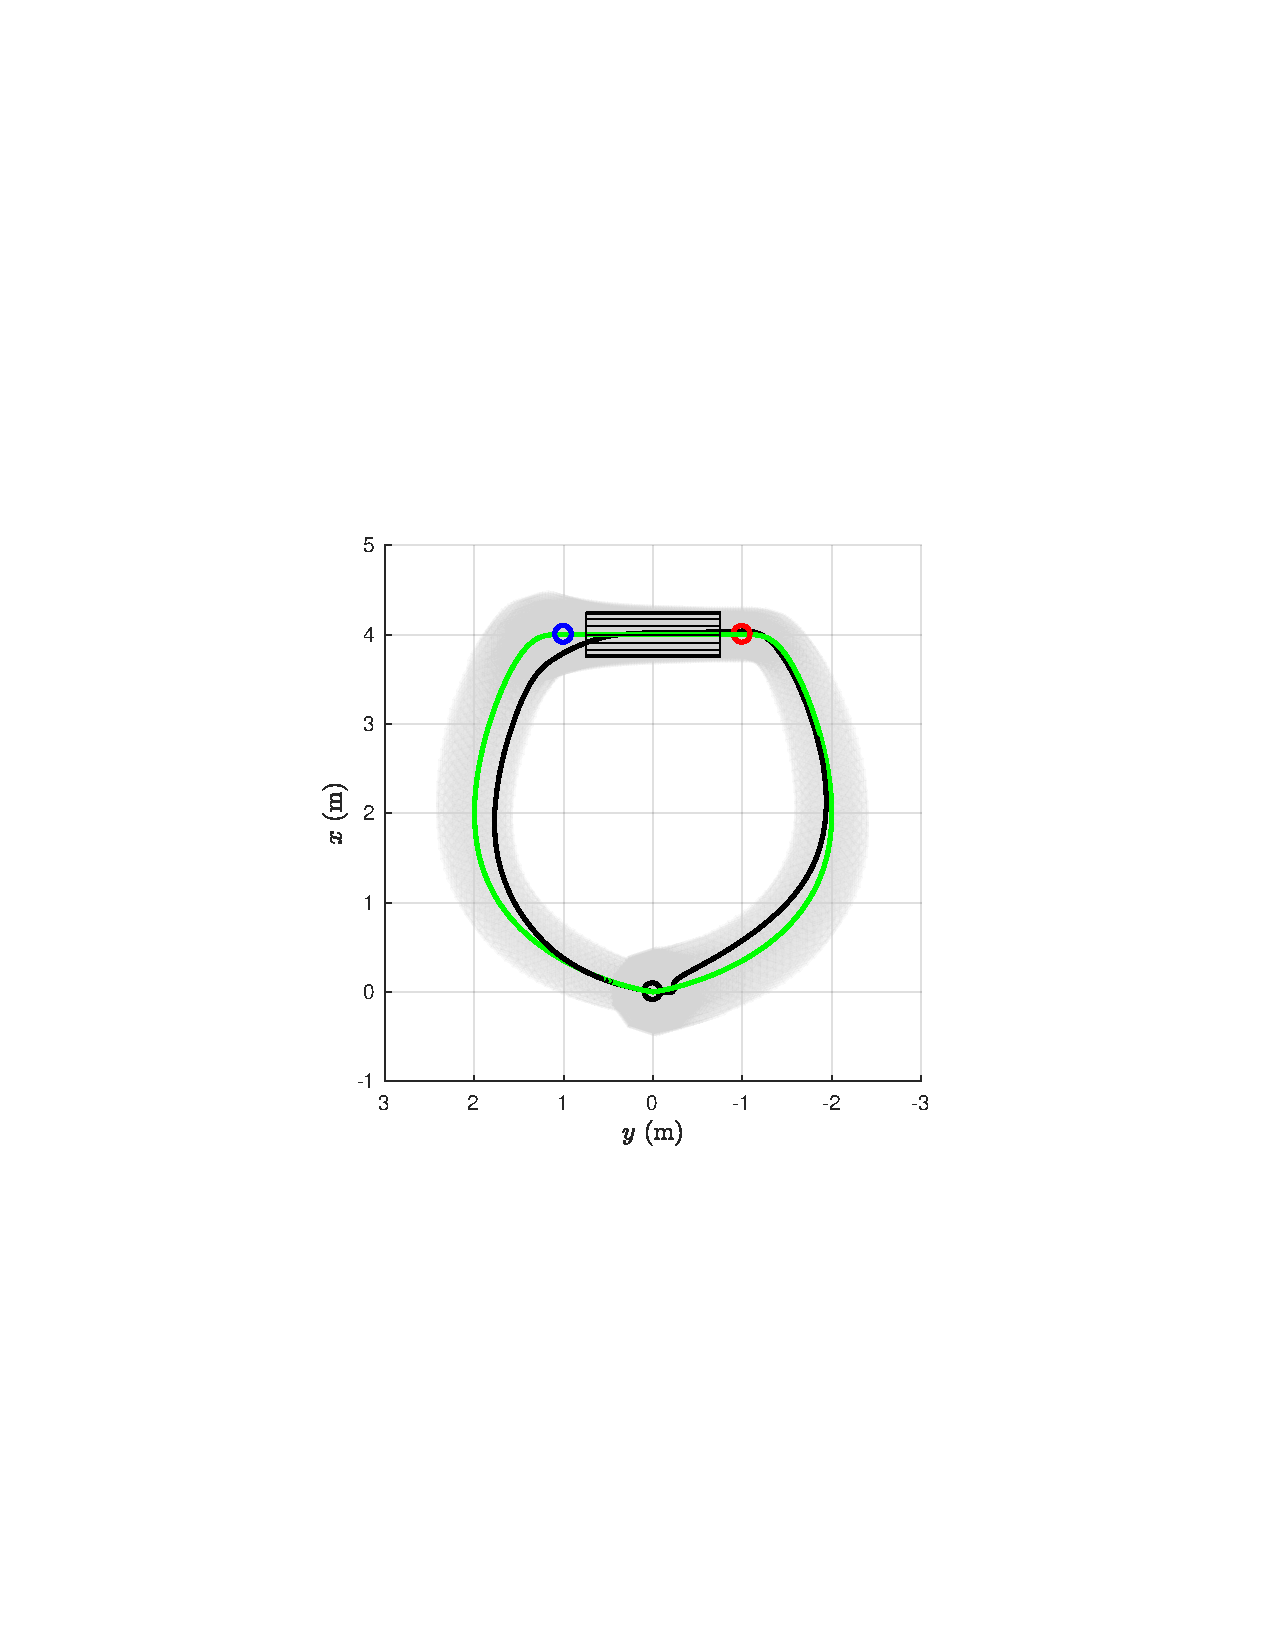
\includegraphics[width=9.0cm]{slow.pdf}
\caption{The reference speed between the blue and red points is $1.0$ m/s.}
\end{subfigure}
\begin{subfigure}[b]{0.5\textwidth}
\centering
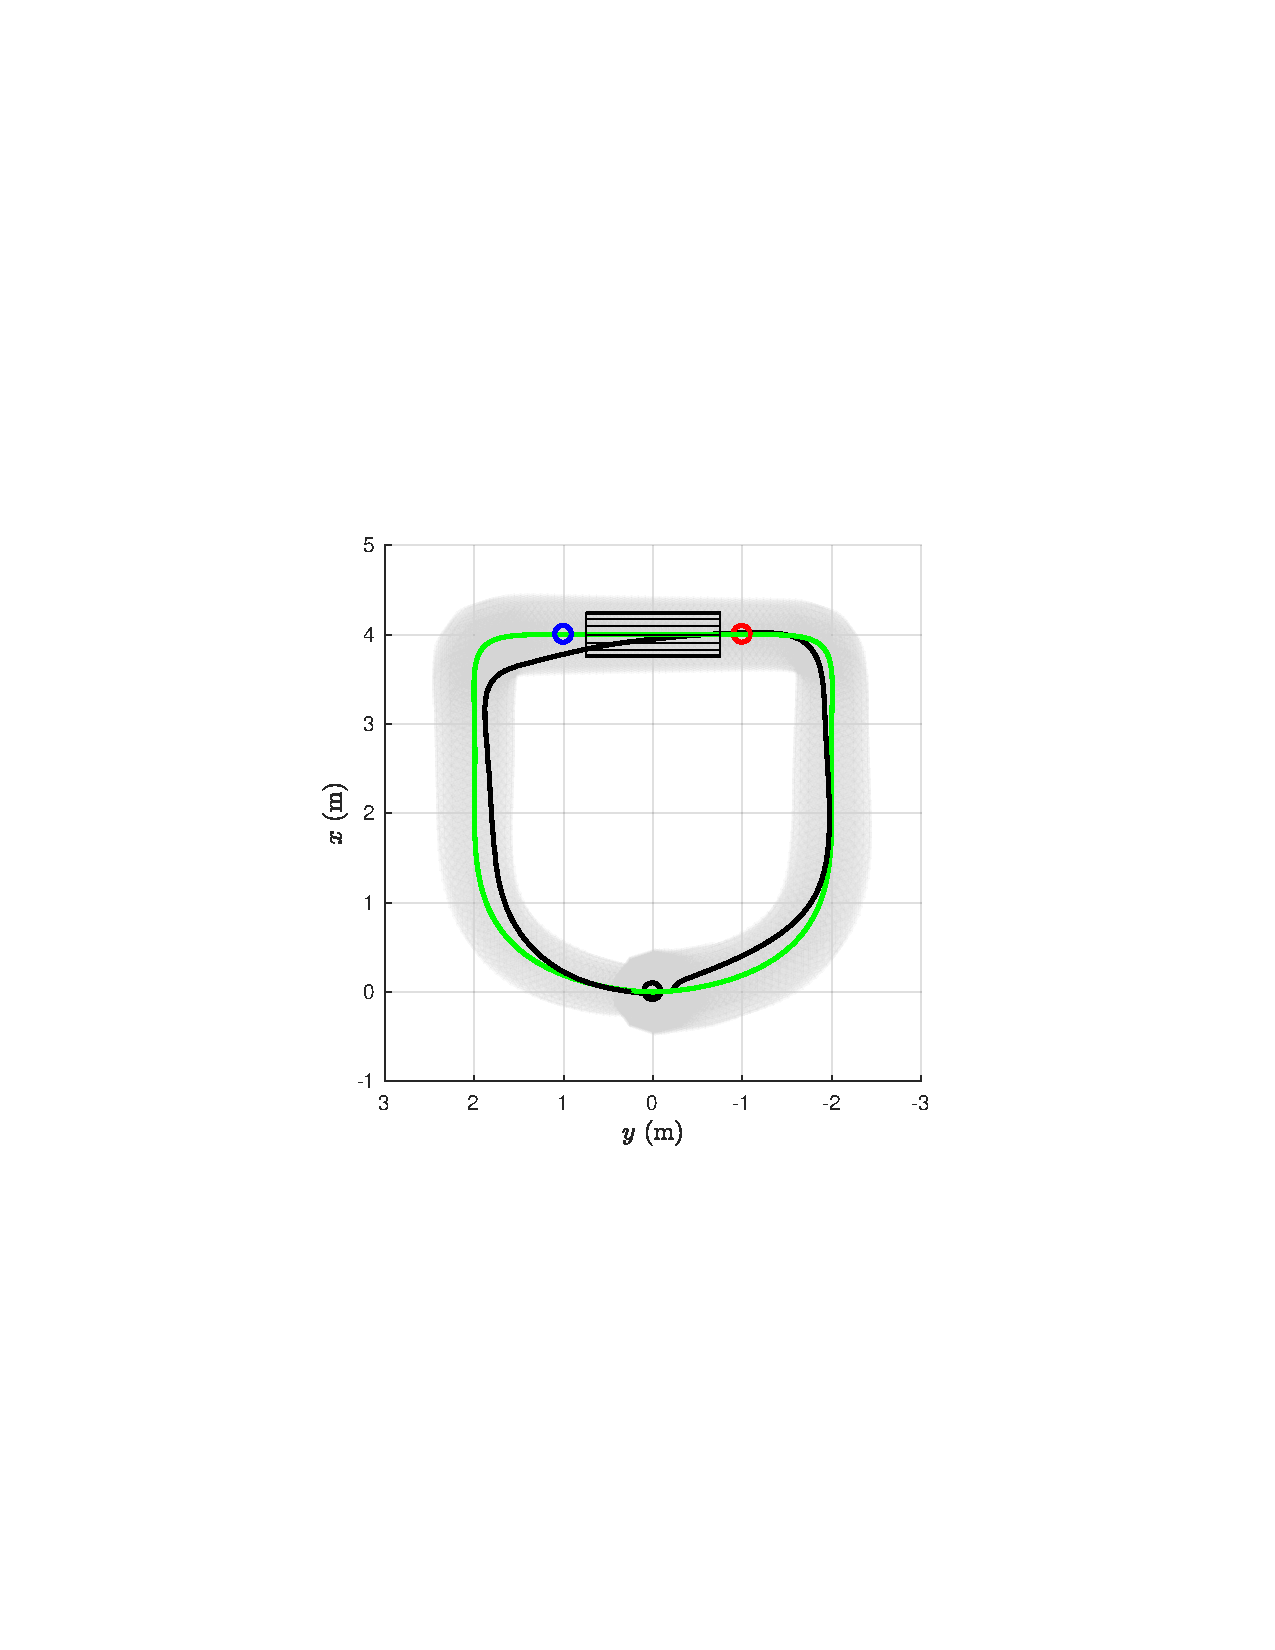
\includegraphics[width=9.0cm]{fast.pdf}
\caption{The reference speed between the blue and red points is $2.6$ m/s.}
\end{subfigure}
\caption{The green and black lines are the reference and measured trajectories, respectively. The shaded regions represent the funnels around the reference trajectory. The goal of this experiment is to move inside of the pipe between the blue and red points safely.}
\label{fig:experimentalResult}
\end{figure*}

\section{CONCLUSIONS}


%\addtolength{\textheight}{-12cm}   % This command serves to balance the column lengths
%                                  % on the last page of the document manually. It shortens
%                                  % the textheight of the last page by a suitable amount.
%                                  % This command does not take effect until the next page
%                                  % so it should come on the page before the last. Make
%                                  % sure that you do not shorten the textheight too much.

%%%%%%%%%%%%%%%%%%%%%%%%%%%%%%%%%%%%%%%%%%%%%%%%%%%%%%%%%%%%%%%%%%%%%%%%%%%%%%%%



%%%%%%%%%%%%%%%%%%%%%%%%%%%%%%%%%%%%%%%%%%%%%%%%%%%%%%%%%%%%%%%%%%%%%%%%%%%%%%%%



%%%%%%%%%%%%%%%%%%%%%%%%%%%%%%%%%%%%%%%%%%%%%%%%%%%%%%%%%%%%%%%%%%%%%%%%%%%%%%%%

\section*{ACKNOWLEDGMENT}


%%%%%%%%%%%%%%%%%%%%%%%%%%%%%%%%%%%%%%%%%%%%%%%%%%%%%%%%%%%%%%%%%%%%%%%%%%%%%%%%


\begin{thebibliography}{99}

\bibitem{c1} G. O. Young, ÒSynthetic structure of industrial plastics (Book style with paper title and editor),Ó 	in Plastics, 2nd ed. vol. 3, J. Peters, Ed.  New York: McGraw-Hill, 1964, pp. 15Ð64.
%\bibitem{c2} W.-K. Chen, Linear Networks and Systems (Book style).	Belmont, CA: Wadsworth, 1993, pp. 123Ð135.
%\bibitem{c3} H. Poor, An Introduction to Signal Detection and Estimation.   New York: Springer-Verlag, 1985, ch. 4.
%\bibitem{c4} B. Smith, ÒAn approach to graphs of linear forms (Unpublished work style),Ó unpublished.
%\bibitem{c5} E. H. Miller, ÒA note on reflector arrays (Periodical styleÑAccepted for publication),Ó IEEE Trans. Antennas Propagat., to be publised.
%\bibitem{c6} J. Wang, ÒFundamentals of erbium-doped fiber amplifiers arrays (Periodical styleÑSubmitted for publication),Ó IEEE J. Quantum Electron., submitted for publication.
%\bibitem{c7} C. J. Kaufman, Rocky Mountain Research Lab., Boulder, CO, private communication, May 1995.
%\bibitem{c8} Y. Yorozu, M. Hirano, K. Oka, and Y. Tagawa, ÒElectron spectroscopy studies on magneto-optical media and plastic substrate interfaces(Translation Journals style),Ó IEEE Transl. J. Magn.Jpn., vol. 2, Aug. 1987, pp. 740Ð741 [Dig. 9th Annu. Conf. Magnetics Japan, 1982, p. 301].
%\bibitem{c9} M. Young, The Techincal Writers Handbook.  Mill Valley, CA: University Science, 1989.
%\bibitem{c10} J. U. Duncombe, ÒInfrared navigationÑPart I: An assessment of feasibility (Periodical style),Ó IEEE Trans. Electron Devices, vol. ED-11, pp. 34Ð39, Jan. 1959.
%\bibitem{c11} S. Chen, B. Mulgrew, and P. M. Grant, ÒA clustering technique for digital communications channel equalization using radial basis function networks,Ó IEEE Trans. Neural Networks, vol. 4, pp. 570Ð578, July 1993.
%\bibitem{c12} R. W. Lucky, ÒAutomatic equalization for digital communication,Ó Bell Syst. Tech. J., vol. 44, no. 4, pp. 547Ð588, Apr. 1965.
%\bibitem{c13} S. P. Bingulac, ÒOn the compatibility of adaptive controllers (Published Conference Proceedings style),Ó in Proc. 4th Annu. Allerton Conf. Circuits and Systems Theory, New York, 1994, pp. 8Ð16.
%\bibitem{c14} G. R. Faulhaber, ÒDesign of service systems with priority reservation,Ó in Conf. Rec. 1995 IEEE Int. Conf. Communications, pp. 3Ð8.
%\bibitem{c15} W. D. Doyle, ÒMagnetization reversal in films with biaxial anisotropy,Ó in 1987 Proc. INTERMAG Conf., pp. 2.2-1Ð2.2-6.
%\bibitem{c16} G. W. Juette and L. E. Zeffanella, ÒRadio noise currents n short sections on bundle conductors (Presented Conference Paper style),Ó presented at the IEEE Summer power Meeting, Dallas, TX, June 22Ð27, 1990, Paper 90 SM 690-0 PWRS.
%\bibitem{c17} J. G. Kreifeldt, ÒAn analysis of surface-detected EMG as an amplitude-modulated noise,Ó presented at the 1989 Int. Conf. Medicine and Biological Engineering, Chicago, IL.
%\bibitem{c18} J. Williams, ÒNarrow-band analyzer (Thesis or Dissertation style),Ó Ph.D. dissertation, Dept. Elect. Eng., Harvard Univ., Cambridge, MA, 1993. 
%\bibitem{c19} N. Kawasaki, ÒParametric study of thermal and chemical nonequilibrium nozzle flow,Ó M.S. thesis, Dept. Electron. Eng., Osaka Univ., Osaka, Japan, 1993.
%\bibitem{c20} J. P. Wilkinson, ÒNonlinear resonant circuit devices (Patent style),Ó U.S. Patent 3 624 12, July 16, 1990. 
%





\end{thebibliography}




\end{document}

